\begin{frame}
\frametitle{Stability}
\begin{center}
$\Delta t = 0.001 \longrightarrow \Delta t = 0.002$

\includegraphics[scale=0.27]{../check/stable_001.png}

\includegraphics[scale=0.27]{../check/unstable_002.png}
\end{center}
\end{frame}

\begin{frame}[fragile]
\frametitle{Performances}
\framesubtitle{GPU}
\begin{lstlisting}
Device 0: "GeForce GTX 780"

CUDA Driver Version / Runtime Version          8.0 / 6.5
CUDA Capability Major/Minor version number:    3.5
Total amount of global memory:                 3071 MBytes
(12) Multiprocessors, (192) CUDA Cores/MP:     2304 CUDA Cores
GPU Clock rate:                                941 MHz
Memory Clock rate:                             3004 Mhz
Memory Bus Width:                              384-bit
L2 Cache Size:                                 1572864 bytes

Total amount of constant memory:               65536 bytes
Total amount of shared memory per block:       49152 bytes
Total number of registers available per block: 65536
Warp size:                                     32
Maximum number of threads per multiprocessor:  2048
Maximum number of threads per block:           1024
\end{lstlisting}
\begin{center}

\end{center}
\end{frame}

\begin{frame}
\frametitle{Performances}
\framesubtitle{Execution time}
\begin{center}
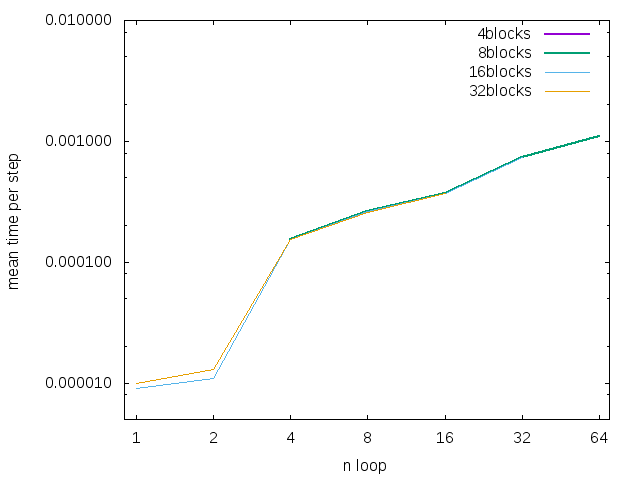
\includegraphics[scale=0.5]{../check/time/speed.png}
\end{center}
\end{frame}

\begin{frame}
\frametitle{Performances}
\framesubtitle{Execution time GPU vs CPU}
\begin{center}
%
\includegraphics[scale=0.4]{../check/borders_1c_01.png}
\end{center}
\end{frame}

\begin{frame}
\frametitle{Performances}
\framesubtitle{Different GPUs}
\begin{center}
\begin{tabular}{l l r}
GeForce GTX 960		&	(sandy1)	&	$8.3\pm0.1\times10^{-5}$ s\\
GeForce GTX 780		&	(sandy2)	&	$8.5\pm0.2\times10^{-5}$ s\\
GeForce GTX 470		&	(seven1)	&	$1.1\pm0.2\times10^{-4}$ s\\
GeForce GTX 560 Ti	&	(seven4)	&	$1.12\pm0.03\times10^{-4}$ s\\
-	&	(seven3)	&	n.w.\\
GeForce 210			&	(seven5)	&	n.w.\\
\end{tabular}
\end{center}
\end{frame}
